\documentclass[11pt, oneside]{article} 
\usepackage{geometry}
\geometry{letterpaper} 
\usepackage{graphicx}
	
\usepackage{amssymb}
\usepackage{amsmath}
\usepackage{parskip}
\usepackage{color}
\usepackage{hyperref}

\graphicspath{{/Users/telliott_admin/Dropbox/Tex/png/}}
% \begin{center} 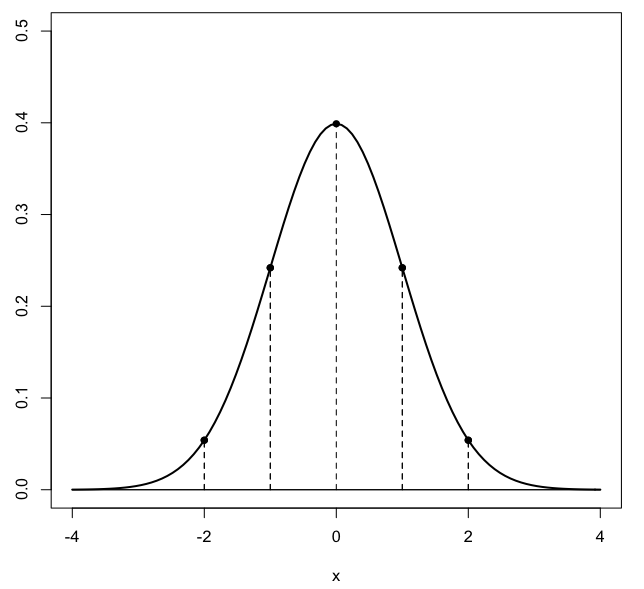
\includegraphics [scale=0.4] {gauss3.png} \end{center}

\title{Continuity}
\date{}

\begin{document}
\maketitle
\Large

Continuity has an intuitive definition:  if we can graph a function \emph{without lifting our pencil from the paper}, then the function is continuous.

Here are some graphs showing examples of how continuity can fail.
\begin{center} 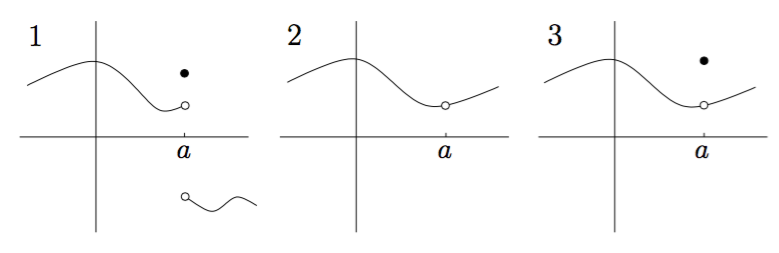
\includegraphics [scale=0.5] {continuity_failure.png} \end{center}
\begin{center} 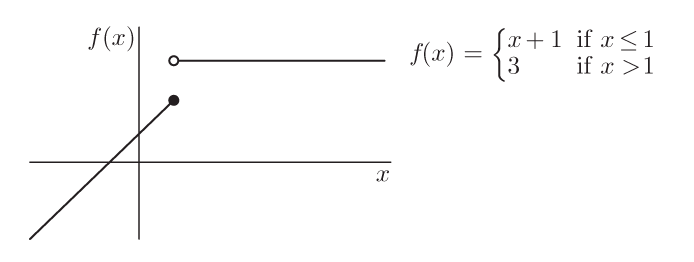
\includegraphics [scale=0.5] {continuity_failure2.png} \end{center}

For a function to be continuous at a point $x=c$, we imagine that if we vary $x$ in neighborhood of $c$, then $f(x)$ should not change in value by too much.

Again, we will call that value $L$, the limit of $f(x)$ as $x \rightarrow c$.  For $L$ to exist we require that the two one-sided limits be equal.  

In addition, it must also be true that $f(c) = L$.

\subsection*{fancy definition}
If we had not previously developed the concept of a limit, we might proceed as follows:  a function $f : \mathbb{R} \rightarrow \mathbb{R}$ is continuous at $c \in \mathbb{R}$ if and only if
\[ \forall \ \epsilon > 0 \ \exists \ \delta > 0 \ \text{ such that, if } |x-c| < \delta, \text{ then } |f(x) - f(c)| < \epsilon \]

\subsection*{example:  absolute value}
An algebraic definition of the absolute value function is piecewise:
\[ |x| =
\begin{cases}
\ \ x, \ \ \ x \ge 0  \\
-x, \ \ \ x < 0
\end{cases}
\]
\begin{center} 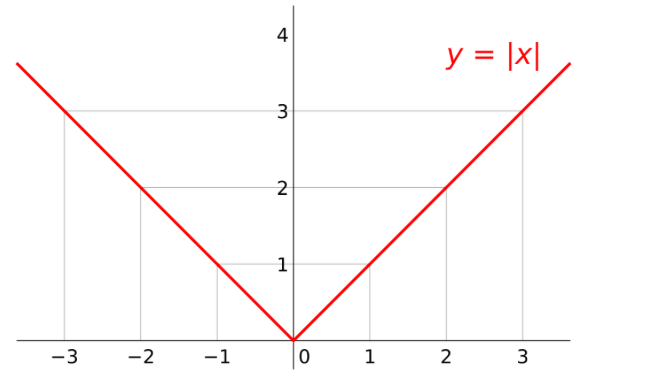
\includegraphics [scale=0.4] {abs.png} \end{center}
The function $f(x) = |x|$ is continuous at $x=0$ because the two one-sided limits exist and are equal to each other.  They are also equal to $f(0) = 0$.

\subsection*{example:  constant}
Suppose $f(x) = a$ for some real number $a$.  Then no matter what $\epsilon$ is chosen and no matter what real number $c$ is chosen
\[ f(x) = f(c) = a \]
so
\[ |f(x) - f(c)| < \epsilon \]

\subsection*{example:  x}
Suppose $f(x) = x$.  
\[ \lim_{x \rightarrow c} f(x) = c  = f(c) \]
so $f$ is continuous at $c$.

Or choose $\delta = \epsilon$.  Then, if $|x-c| < \delta$
\[ c- \delta < x < c + \delta \]
\[ f(x) = x \]
\[ f(x) - c < \delta = \epsilon \]
\[ | f(x) - c | < \epsilon \]
so $f$ is continuous at $c$

\subsection*{example:  constant factor}
Suppose $f(x) = cx$ ($c \in \mathbb{R}$).  Use the $\epsilon-\delta$ game to prove that $f$ is continuous.

Proof:  the function "stretches" $x$ by a factor of $c$.  Hence $\delta$ will also be stretched.  Set $\delta = \epsilon/c$.  Then, if $|x-a| < \delta$ we have
\[ |f(x) - f(a)| = |cx - ca| = c |x-a| < c \delta = c \epsilon / c = \epsilon \]
Hence $f$ is continuous at every $a \in \mathbb{R}$.

\subsection*{example:  product rule}
How to prove that $f(x) = x^2$ is continuous?  One way is to try adjusting $\delta$ based on the value of $a$ (e.g. min $(| \sqrt{a^2 + \epsilon} \ \pm a|)$), but a better way is to invoke the product rule.

If $f: \mathbb{R} \rightarrow \mathbb{R}$ and $g: \mathbb{R} \rightarrow \mathbb{R}$ are both continuous at $a \in  \mathbb{R}$, then $fg$ is continuous at $a$.

First, prove $f(x) = x$ is continuous.  Then define $f(x) = g(x) = x$.  So $x^2 = f(x) g(x)$ in continuous.

By induction then, all powers $f(x) = x^n$ are continuous.

\subsection*{proof of the product rule for continuity}
Let $f$ and $g$ be functions defined on an open subset of $\mathbb{R}$.  We have that $f$ and $g$ are both continuous at $c$ which means that
\[ \lim_{x \rightarrow c} f(x) = L \]
\[ \lim_{x \rightarrow c} g(x) = M \]
Then
\[ \lim_{x \rightarrow c} f(x) \cdot g(x) = \lim_{x \rightarrow c} f(x) \cdot \lim_{x \rightarrow c} g(x) = LM \]

To obtain this result we have used the product rule for limits. 

\subsection*{example:  inverse}
Consider the function $f(x) = 1/x$.  Above we pointed out that this function is undefined at $x=0$ since division by zero is not defined.  But there is nothing to stop us from defining the function piecewise, like so:

\[ f(x) = 
\begin{cases}
\frac{1}{x} \ \ x \ne 0 \\
0 \ \ x = 0 
\end{cases} \]

As $x$ gets close to zero from the right, $1/x$ continues to take on larger and larger positive values, but then dives to $0$ at $x=0$ and then further dives toward $-\infty$ as we pass to the left of zero.

Trick question:  give an example of a function $f : \mathbb{R} \rightarrow \mathbb{R}$ that is not continuous at zero.  If you said the inverse, that is not correct.  The reason is that the inverse is not $f : \mathbb{R} \rightarrow \mathbb{R}$ because \emph{it is not defined at zero}.

On the other hand, $f(x) = \sin(x)$ \emph{is} $f : \mathbb{R} \rightarrow \mathbb{R}$ even though the values actually output by the function are $f(x) \in [-1,1]$.  That interval is the \emph{image} of the function, any codomain so that the image is contained in the codomain will do.

\subsection*{example}
A famous (but weird) function is defined as
\[ f(x) =
\begin{cases}
1 \ \ \text{ if } x \in \mathbb{Q} \\
0 \ \ \text{ if } x \notin \mathbb{Q} 
\end{cases}
\]

As we said before, you can imagine that the graph of this function looks like a linear hairbrush, with spikes at each rational number.

However, any interval such as $[0,1]$, or $[0.001, 0.002]$ contains an infinite number of rational numbers, but an even larger infinite number of real numbers.  In other words, we only get the hairbrush image if we exclude denominators greater than some value.  And we get the exact same image if we blow up any portion of the graph.

This is hard to think about.

The first function is not continuous anywhere, but the following variant is:
\[ f(x) =
\begin{cases}
x \ \ \text{ if } x \in \mathbb{Q} \\
0 \ \ \text{ if } x \notin \mathbb{Q} 
\end{cases}
\]

Why?

\subsection*{uniform continuity}
The notion of continuity described so far is called "pointwise."  We first pick a point $c$, and then working near that point, we pick an $\epsilon$ and then a $\delta$ and so on.  A particular $\delta$ may be satisfactory for some values of $c$ and not for others.

One can pick a "one-size-fits-all" $\delta$ for some functions and intervals, but not always.  

Weierstrass and his student Heine developed the idea of "uniform continuity".

\begin{center} 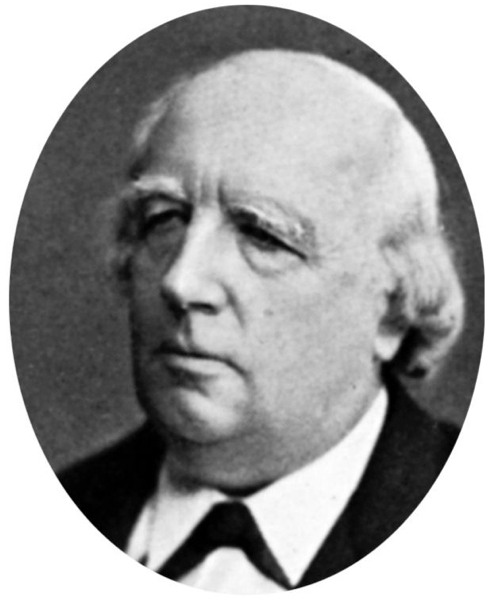
\includegraphics [scale=0.4] {Weierstrass} \end{center}
Weierstrass

A function $f$ is uniformly continuous on some domain if, for every $\epsilon > 0$, there exists a $\delta > 0$ so that, if $x$ and $y$ are any two points in the domain within $\delta$ units of one another, then $|f(x) - f(y)| < \epsilon$.  This $\delta$ must work everywhere in the domain.

It turns out that a function can be point-wise but not uniformly continuous.  Consider $f(x) = 1/x$ on the open interval $(0,1)$.  The problem is that the values of the function rise to $\infty$ as $x \rightarrow 0$.  Suppose you have some $\delta$ that works for a particular $\epsilon$ near point $c$.  We can always move far enough to the left to a new pair $x,y$ so that the rise in $f(x)$ for a change in $x$ of $\delta$ is $> \epsilon$.

However, Heine proved that a function continous on a closed, bounded interval $[a,b]$ must be uniformly continuous.  According to the internet, 
"a function is uniformly continuous on $(0,1)$ if and only if it can be extended continuously to $[0,1]$."

\end{document}  